% Air‑Quality Platform Poster (baposter)
\documentclass[a0paper,portrait]{baposter}

% ---------- Encoding & Fonts ----------
\usepackage[utf8]{inputenc}
\usepackage[T1]{fontenc}
\usepackage[english]{babel}
\usepackage{helvet}
\renewcommand{\familydefault}{\sfdefault}
\usepackage[helvet]{sfmath}

% ---------- Graphics & Figures ----------
\usepackage{graphicx}
\usepackage{caption}
\captionsetup{font=small,labelfont=bf}

% ---------- Mathematics ----------
\usepackage{amsmath,amssymb}
\usepackage{booktabs}

% ---------- Color Palette ----------
\selectcolormodel{RGB}
\definecolor{udblue}{RGB}{0,70,120}
\definecolor{udgray}{RGB}{230,230,235}

% ---------- Macros ----------
\newcommand{\alert}[1]{{\color{udblue}#1}}

% ---------- Background ----------
\background{
  \begin{tikzpicture}[remember picture,overlay]
    \fill[fill=udgray] (current page.north west) rectangle (current page.south east);
    \fill[fill=udblue] (current page.north west) rectangle ([yshift=-0.1\textheight] current page.north east);
  \end{tikzpicture}
}

% ---------- Poster Setup ----------
\begin{document}
\begin{poster}{
  grid=false,
  columns=2,
  headerheight=0.1\textheight,
  background=none,
  headerborder=closed,
  borderColor=udblue,
  headershape=rectangle,
  headerColorOne=udblue,
  headerFontColor=white,
  headerfont=\Large\bfseries,
  boxColorOne=white,
  textborder=rectangle,
  linewidth=1pt
}
{
  % Eye‑catcher logo (replace with university logo if desired)
  
\includegraphics[height=0.9\headerheight]{images/logo_escudo_vertical.png}
}
% ---- Title ----
{\Large\bf Architecture for Real‑Time Air Quality Monitoring\\and Personalized Recommendations}
% ---- Authors ----
{\small
  Johan~Esteban~Castaño~Martínez, Stivel~Pinilla~Puerta, Jose~Alejando~Cortazar\\
  Systems Engineering Program — Faculty of Engineering\\
  Universidad Distrital Francisco José de Caldas, Bogotá, Colombia\\
  \texttt{jecastanom@udistrital.edu.co}, \texttt{spinillap@udistrital.edu.co}, \texttt{jacortazarl@udistrital.edu.co}
}
{
  % Conference or sponsor logo (optional)
  
\includegraphics[height=0.75\headerheight]{images/identidad facultad-02.png}
}

% ---------- CONTENT BOXES ----------

\begin{posterbox}[name=intro,column=0,row=0]{Introduction}
\begin{itemize}
  \item Air pollution kills \textasciitilde7--8~million people annually and ranks as the \alert{second leading risk factor} for mortality, ahead of high blood pressure or smoking.
  \item In \alert{Bogotá}, PM$_{2.5}$ levels declined from 15.7~\textmu g/m$^3$ (2017) to 13.1~\textmu g/m$^3$ (2019), yet spatially heterogeneous hot spots persist despite Air Plan 2030.
  \item Public APIs (AQICN, Google Air Quality, IQAir) provide real-time data but lack \alert{personalized recommendations} and unified integration for citizen-oriented decision support.
\end{itemize}
\end{posterbox}

\begin{posterbox}[name=goal,column=0,below=intro]{Research Goal}
\begin{itemize}
  \item \textbf{Research Question:} How can we deliver highly‑available, low‑latency air‑quality insights that adapt to user context (location, activity, health risk) in real time?
  \item \textbf{Objective:} Design and validate a PostgreSQL+TimescaleDB architecture that ingests multi‑source AQI streams every 10~min, normalizes heterogeneous payloads, and produces \alert{personalized health recommendations} within 2~s (p95) under 1000 concurrent users.
\end{itemize}
\end{posterbox}

\begin{posterbox}[name=solution,column=0,below=goal]{Proposed Architecture}
\begin{itemize}
  \item \textbf{Ingestor:} Python service polls AQICN, Google Air Quality, and IQAir APIs every 10~min; raw JSON archived in \alert{MinIO} (\texttt{raw-airquality}) for audit and replay.
  \item \textbf{Normalizer:} Stateless mapping layer aligns field names, units, and AQI scales before inserting into \alert{TimescaleDB} hypertable partitioned by \textit{city}$\times$\textit{month}.
  \item \textbf{Query Acceleration:} Concurrently‑refreshed materialized views prevent blocking reads during updates; dashboards access consistent snapshots.
  \item \textbf{Recommendation Engine:} Classifies AQI into EPA bands (Good 0--50, Moderate 51--100, Unhealthy $\geq$151, Hazardous >300) and combines with user metadata (location, activity, risk profile) to generate personalized health advice aligned with WHO guidelines. Suggests certified protective products (N95 masks, air purifiers) when AQI$\geq$151.
  \item \textbf{API Layer:} REST + GraphQL endpoints for citizens, researchers, and administrators; \alert{Grafana} dashboards monitor ingest lag, query latency, and view-refresh duration.
\end{itemize}
  \centering
  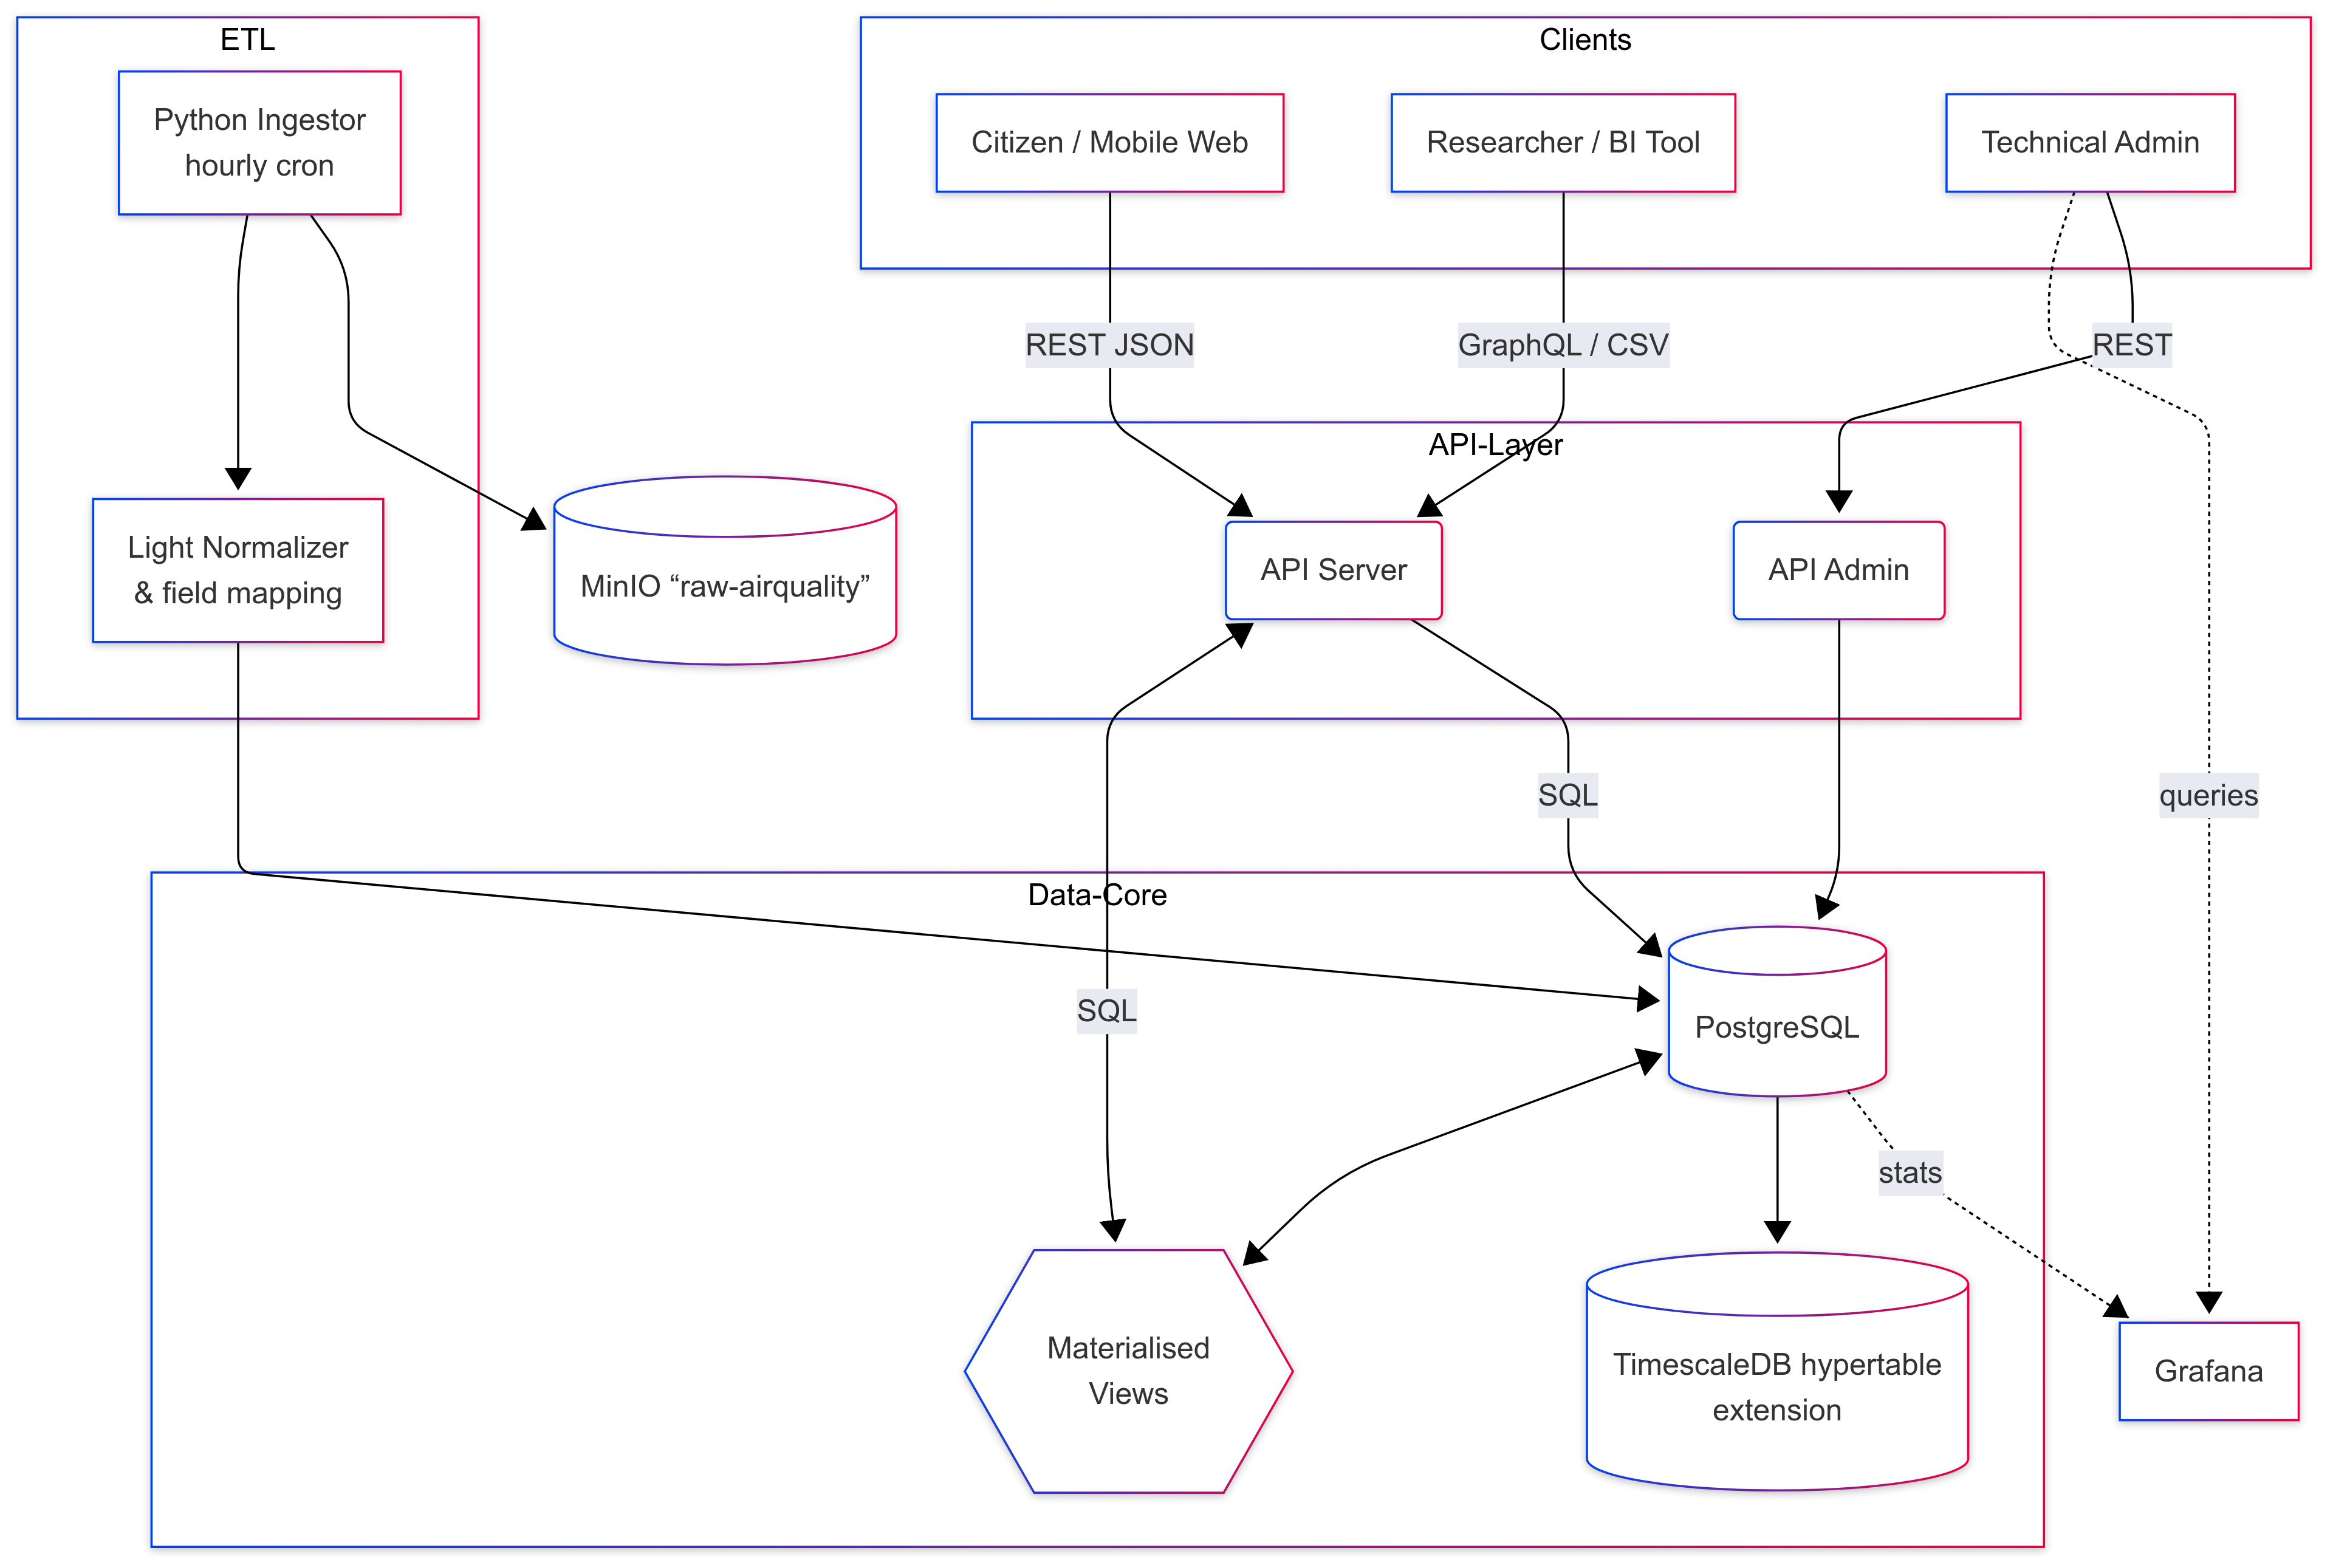
\includegraphics[width=0.95\linewidth]{images/fig1_architecture.png}
  \captionof{figure}{End‑to‑end architecture with three-layer data model (Geospatial, Customer, Recommendation Engine).}
\end{posterbox}

\begin{posterbox}[name=experiments,column=1]{Experimental Setup}
\begin{itemize}
  \item \textbf{Dataset:} AQICN historical CSV (2015--2024). Phase~1 loads 2022--2024 Bogotá data (\textasciitilde2.5M rows/month under current ingestion rates).
  \item \textbf{Hardware:} Primary DB node: 4~vCPU, 16~GB RAM, NVMe storage; MinIO object storage for raw JSON archives.
  \item \textbf{Software:} PostgreSQL 17.1, TimescaleDB 2.14, Python 3.12, Grafana 11.
  \item \textbf{Load Test:} Apache JMeter simulates 1000 concurrent users, each issuing \textasciitilde5 REST/GraphQL requests per second over a 10-minute test window.
  \item \textbf{Metrics:} Query latency (NFR1), dashboard load time (NFR6), report generation (NFR4), recommendation update frequency (NFR5), materialized-view refresh, CPU utilization, system uptime (NFR7).
\end{itemize}
\end{posterbox}

\begin{posterbox}[name=results,column=1,below=experiments]{Target Performance Metrics}
\begin{center}
\begin{tabular}{lcc}
\toprule
\textbf{Metric} & \textbf{Target (p95)} & \textbf{Requirement}\\
\midrule
Query latency ($\geq$1M rows) & $\leq$2~s & NFR1, NFR3\\
Dashboard load time & $\leq$2~s & NFR6, US12\\
Report generation & $\leq$10~s & NFR4\\
Recommendation update & 10~min & NFR5\\
Materialized-view refresh & $\leq$5~s & Near real-time\\
Concurrent users & 1000 users & US13, NFR8\\
System uptime & $\geq$99.9\% & NFR7, US14\\
Peak CPU utilization & $<$70\% & Headroom\\
\bottomrule
\end{tabular}
\end{center}
\vspace{0.5em}
Targets aligned with functional (FR1--FR14) and non-functional (NFR1--NFR10) requirements defined in project specification.
\end{posterbox}

\begin{posterbox}[name=conclusion,column=1,below=results]{Conclusions and Future Work}
\textbf{Key Contributions:}
\begin{itemize}
  \item \alert{End-to-end PostgreSQL-based architecture} unifying three public APIs with 10-min refresh cycles, MinIO raw storage, and monthly city-partitioned TimescaleDB hypertables.
  \item \alert{Lightweight recommendation engine} translating AQI thresholds + user context into personalized health advice and certified product suggestions (FR8--FR11).
  \item \alert{Target performance:} sub-2~s latency (p95) for 1000 concurrent users without distributed streaming frameworks (Kafka/Flink).
\end{itemize}
\textbf{Future Directions:}
\begin{itemize}
  \item Predictive analytics: ARIMAX/LSTM forecasts for 6--24h pollution peaks.
  \item Performance optimization: read replicas, Redis caching, message queue (RabbitMQ/Kafka) for asynchronous ingestion.
  \item Geographic expansion: multi-region deployment across Latin American cities (Medellín, Cali, Santiago, Lima) using PostgreSQL 17 logical replication.
\end{itemize}
\end{posterbox}

\begin{posterbox}[name=refs,column=1,below=conclusion]{References}
\scriptsize
\begin{thebibliography}{9}
\itemsep=-0.2em
\bibitem{who2021} WHO, "Global Air Quality Guidelines", 2021.
\bibitem{state2024} State of Global Air, "Report 2024", 2024.
\bibitem{aqicn} AQICN, "Real-Time Air Quality Index API", 2024.
\bibitem{google} Google, "Air Quality API Overview", 2024.
\bibitem{iqair} IQAir, "AirVisual API Documentation", 2024.
\bibitem{timescale} Timescale Inc., "Tables and Hypertables", 2025.
\bibitem{postgsmv} PostgreSQL, "REFRESH MATERIALIZED VIEW", Docs.
\bibitem{minio} MinIO Inc., "Object Storage for Linux", 2024.
\bibitem{grafana} Grafana Labs, "Dashboards Overview", 2024.
\end{thebibliography}
\end{posterbox}

\end{poster}
\end{document}
